%# -*- coding: utf-8-unix -*-
%%==================================================
%% chapter0.tex for SJTU Master Thesis
%%==================================================


\chapter{智能温室监测与控制系统}
\label{chapter:IntelligentGreenhouseSystem}
基于智能温室系统的四层架构设计和各层次的概要设计,本章分别对系统中的感知控制层、网络传输层、应用层和终端接入层进行了详细地设计与实现,并最终完成了智能温室监测与控制系统。

\section{感知控制层设计与实现}
	\subsection{传感器网络选择}
	温室内应用环境特殊,通常可供布置传感器的空间有限、温室内种植植物导致布线困难、温室面积较大从而监测范围大、农业生产环境不易值守且维护不便,传统的有线传感器网络对于温室内环境的监测不是一个很好的选择。针对温室内环境监测传感器布置困难、供电困难、搭建和维护成本限制大等因素,综合考虑,本系统对于温室内环境监测选用ZigBee无线传感器网络。

	ZigBee技术是一种基于IEEE 802.15.4标准的局域网通信技术,是WSNs信息采集系统的一个重要组成部分,主要用于传感测量和控制应用,具有低功耗、低成本、复杂度低、短延迟、高容量、高安全性、自组网、可灵活扩展、使用免执照频段等优良性能。

	由于系统内室外环境监测使用的微型气象站和太阳辐射传感器安装部署位置固定,不存在温室内传感器测点所存在的问题,因此采用具有抗噪能力强、传输距离长、实现成本低和具有多站能力的RS485有线传感器网络。

	两种网络均通过USB转串口与上层系统连接通讯。
	\subsection{传感器网络硬件组成}
	温室内无线传感器网络有三种类型的设备组成,分别为传感器节点、路由器节点和协调器。各节点的硬件设计采用模块化设计,各功能模块独立设计,然后通过标准化的接口连接组合成完整的节点,这样既便于维护和升级,同时可以减少主板体积。一个完整节点主要包括核心板模块、传感器模块和底板,其中传感器节点和路由器节点包含所有模块,协调器节点不包含传感器模块。
		\subsubsection{核心板模块}
		核心板由Texas Instruments公司的CC2530 SoC芯片、外围电路及天线组成,如\ref{fig:CC2530}所示。CC2530是用于2.4GHz IEEE 802.15.4和ZigBee应用的片上解决方案,集成了一块增强型8051MCU和一块射频芯片,具有系统内可编程闪存和8-KB RAM、最大256KB的Flash;结合了TI在业内领先的高性能RF收发器,内置4个不同功能的定时器,高度集成的片上系统提供了丰富的外设,只需少量的外部器件即可开发丰富的应用,满足低功耗设计的需求,适用于温室的控制和测量。
		\begin{figure}[!htp]
  			\centering
 			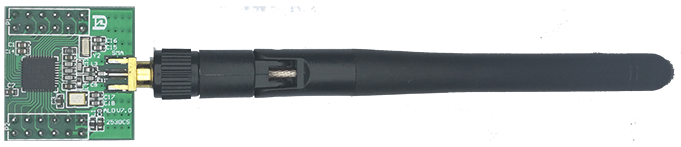
\includegraphics[width=0.5\textwidth]{05CoreBoard.png}
  			\bicaption[fig:CC2530]{CC2530核心板}{CC2530核心板}{Fig}{CC2530 core board}
		\end{figure}
		
		核心板上主要包括CC2530F256单片机、天线接口、晶振、I/O扩展接口等,只需要提供2~3.6V的外部供电并插入天线即可正常工作。
		\subsubsection{传感器模块}
		传感器模块包括空气温湿度传感器、土壤温湿度传感器和照度传感器。
		
		(a) 空气温湿度传感器
		
		温室环境监测需要准确、稳定、线性较好的空气温湿度测量。针对农业生产高温、高湿、高辐射的特殊环境,要求传感器有一定的防水、防尘、抗干扰和低功耗能力。
		
		本系统空气温度测量采用能隙式测温元件,具有响应快、尺寸小、非线性小、低功耗等优点,但不耐高温,适用于中低温区域的环境温度测量,符合温室内空气温度的监测要求;空气湿度测量采用电容聚合体测湿元件,具有灵敏度高、线性度好、稳定性该、响应速度快、重复性较好、温度系数较低等优点,符合温室内空气湿度的监测要求。
 		\begin{figure}[!htp]
  			\centering
 			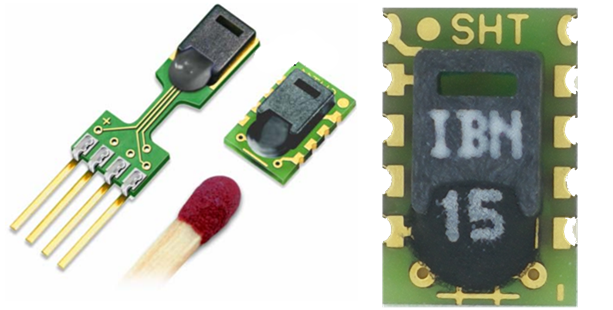
\includegraphics[width=0.3\textwidth]{06SHT15.png}
  			\bicaption[fig:SHT15]{SHT15温湿度传感器}{SHT15温湿度传感器}{Fig}{SHT15 humidity and temperature sensor}
		\end{figure}
		本系统选用SHT15温湿度一体传感器,如\ref{fig:SHT15}所示,集成了温度测量元件、湿度测量元件和ADC,通过串口电路直接输出已校准的数字信号,响应快、可以较好的屏蔽干扰。且其采用2.4~5.5V宽电压供电,可以适应不同的供电要求,休眠时电流低至0.3 ,测量电流仅为550 ,具有良好的低功耗性能,符合温室环境监测低功耗的设计需求。该传感器在室温下测量精度可达到±0.3 ℃和±2\%RH,分辨率8~12 bits可调,量程-40 ℃~123.8 ℃和0~100\%RH,且长期稳定性好,符合温室内空气温度和湿度的测量要求
		
		(b) 土壤温湿度传感器
		
		一般情况下,温室内土壤温湿度分布均匀且变化缓慢,温室环境监测对于土壤温湿度的精度、灵敏度和测量范围要求不高,但是要求有较好的稳定性和线性,同时要可以适应各种复杂的土壤环境。
  		\begin{figure}[!htp]
  			\centering
 			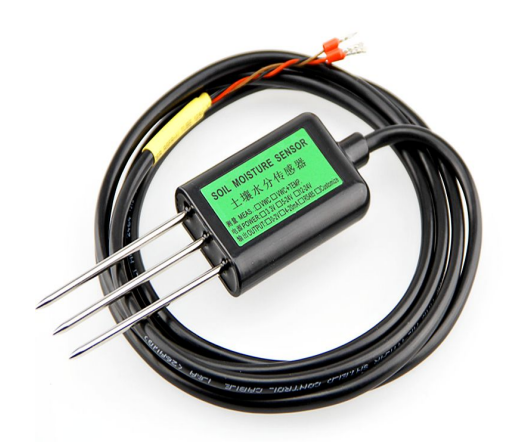
\includegraphics[width=0.3\textwidth]{07SMS50.png}
  			\bicaption[fig:SMS50]{SMS-II-50土壤温湿度传感器}{SMS-II-50土壤温湿度传感器}{Fig}{SMS-II-50 soil moisture and temperature sensor}
		\end{figure}
		本系统选用SMS-II-50土壤水分温度传感器,如\ref{fig:SMS50}所示,集成了一个MS10土壤湿度传感器和一个热电阻温度传感器,包含电源稳压器和防反接电路,采用环氧树脂外壳,可以达到IP68级防护,可直接插入或埋入土壤中,具有良好的抗氧化和耐腐蚀能力,符合温室中恶劣环境的使用需求。具体性能参数如\ref{tab:SMS50}所示。
		
		\begin{table}[!hpb]
  			\centering
  			\bicaption[tab:SMS50]{SMS-II-50性能参数表}{SMS-II-50性能参数表}{Table}{The performance parameters of SMS-II-50}
  			\begin{tabular}{lcc} \toprule
    		参数 & 土壤湿度 & 土壤温度 \\ \midrule
    		输出方式 & \multicolumn{2}{c}{0~2V模拟量/485输出} \\
    		测量量程 & 0~100\%(体积含水量) & -40~80℃\\
			测量精度 & ±5\% & ±0.5℃\\
    		响应时间 & \multicolumn{2}{c}{<1s} \\
    		供电电压 & \multicolumn{2}{c}{3.0~3.6V} \\
    		最大功耗 & \multicolumn{2}{c}{40mA} \\
    		土壤水分监测区域 & \multicolumn{2}{c}{以探针为中心,直径7cm,高度7cm的圆柱形区域} \\
    		防护等级 & \multicolumn{2}{c}{IP68} \\
    		探针和密封材料 & \multicolumn{2}{c}{探针:食用级不锈钢;密封:黑色阻燃环氧树脂} \\
    		安装方式 & \multicolumn{2}{c}{探针全部插入或整体埋入被测介质中} \\ \bottomrule
 			\end{tabular}
		\end{table}

		(c) 光照强度传感器
		
温室中的光照主要来自于太阳辐射和人工光照,光照强度测量范围主要为可见光波段。本文选用BH1750FVI光照强度传感器,具备I2C接口可以输出数字信号,采用高精度宽频谱的光电二极管,内置16bit ADC,在1-65535 lx的量程范围内具有平均分辨率1 lx,2.4~3.6V宽电压供电,成本和功耗低,可自动过滤50Hz/60Hz光噪声干扰,抗干扰能力强,适用于温室环境监测中应用。

		\subsubsection{底板模块}
		底板主要包括电源管理模块和接口模块。电源管理模块包含太阳能电池板与内置电池充电放电管理模块,以及传感器供电管理模块,通过收集温室环境能源即太阳能并储存于内置电池实现传感器系统的长期无值守工作。对外接口包括RS485接口、核心板接口和传感器接口。	
		
		\subsubsection{室外微型气象站和太阳辐射传感器}
		智能温室系统不仅需要对温室内的环境进行监测,还需要对室外的环境进行监测,两者结合才能更好地分析温室环境变化,更有效地对温室内环境进行控制。
  		\begin{figure}[!htp]
  			\centering
 			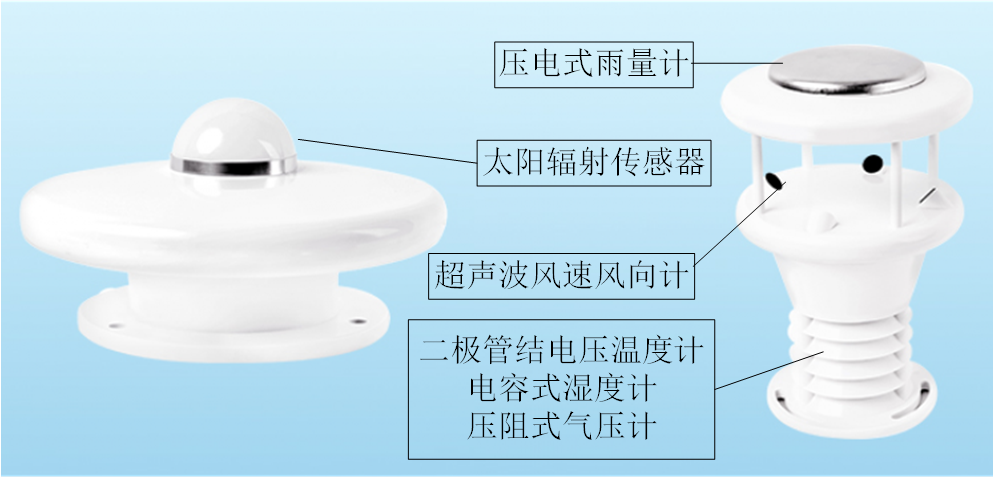
\includegraphics[width=0.8\textwidth]{08WeatherStation.png}
  			\bicaption[fig:WeatherStation]{MULTI-6P六要素微型气象站和GZ-300太阳辐射传感器}{MULTI-6P六要素微型气象站和GZ-300太阳辐射传感器}{Fig}{MULTI-6P 6-elements miniature weather station and GZ-300 solar light intensity meter}
		\end{figure}
		本系统选用智翔宇仪器MULTI-6P 六参数微型气象站和GZ-300 太阳辐射传感器,结构外观如\ref{fig:WeatherStation}所示,可同时测量七种参数,如表2所示。其中微型气象站包括采用超声波风速传感器、风向传感器,压阻式大气压传感器,二极管结电压空气温度传感器,电容式空气湿度传感器,压电式雨量传感器;太阳辐射传感器利用光电效应对太阳辐射强度进行测量;详细参数见\ref{tab:WeatherStation}。微型气象站和太阳辐射传感器都采用一体化设计的金属外壳,抗污染和耐腐蚀性能强,采用紧凑和轻量化结构设计,易于安装拆卸,不需要现场维护和校准,可适应不同的工作环境。两者均采用12-30 V直流电源供电,可同时提供数字和模拟两种信号,其中数字信号输出为RS-485总线输出,供电和信号输入输出均通过底部航空插头,防护等级达到IP65级。
		
		\begin{table}[!hpb]
  			\centering
  			\bicaption[tab:WeatherStation]{MULTI-6P和GZ-300参数}{MULTI-6P和GZ-300参数}{Table}{The performance parameters of the MULTI-6P and GZ-300}
  			\begin{tabular}{ccccc} \toprule
			测量参数 & 测量原理 & 测量范围 & 测量精度 & 分辨率\\ \midrule
			空气温度 & 二极管结电压法 & -40-80 ℃ &	±0.5 ℃ &	0.1 ℃\\
			空气湿度 & 电容式 & 0-100\%RH & ±2\%RH & 0.1\%RH\\
			风速 & 超声波时差法 & 0-60 m/s & ±0.2 m/s & 0.1 m/s\\
			风向 & 超声波时差法 & 0-359.9° & ±3° & 0.1°\\
			大气压 & 压阻式 & 10-1100 hPa	 & ±0.5	 & 0.1 hPa\\
			雨量 & 压电式 & 0-200 mm/h	 & 	0.1 mm/h\\
			太阳辐射 & 光电效应 & 0-2000 W/m2 & ≤3\% & 	1 W/m2\\ \bottomrule
 			\end{tabular}
		\end{table}

	\subsection{ZigBee网络定义}
	ZigBee无线网络中的设备按其功能分为三种,即协调器、路由器和终端节点。协调器是整个无线网络的通讯中心,主要用来组建网络、维护并管理路由器和终端节点入网等行为;路由器负责数据路由和路径选择,可以通过它方便的扩展网络覆盖范围;终端节点主要负责具体的信息采集任务。终端节点和路由器通过无线信道向协调器上报传感数据,协调器再把接收的数据通过RS485总线上传至上层系统。
	
本系统的底层ZigBee无线传感器网络基于Z-Stack协议栈开发,开发人员可以直接调用协议栈提供的API来实现相应的功能而无需深入了解完整的ZigBee协议等,可以极大程度上为开发工作提供便利,减少开发时间。
\begin{figure}[!htp]
    \centering
    \resizebox{6cm}{!}{\begin{tikzpicture}[node distance=2cm]
    \node (pic) [startstop] {开始};
    \node (bg) [io, below of=pic] {接收请求}; 
    \node (pair) [process, below of=bg] {匹配特征点对};
    \node (threshold) [decision, below of=pair, yshift=-0.5cm] {多于阈值};
    \node (clear) [decision, right of=threshold, xshift=3cm] {清晰?};
    \node (capture) [process, right of=pair, xshift=3cm, yshift=0.5cm] {重采};
    \node (matrix_p) [process, below of=threshold, yshift=-0.8cm] {透视变换矩阵};
    \node (matrix_a) [process, right of=matrix_p, xshift=3cm] {仿射变换矩阵};
    \node (reg) [process, below of=matrix_p] {图像修正};
    \node (return) [startstop, below of=reg] {配准结果};
     
    %连接具体形状
    \draw [arrow](pic) -- (bg);
    \draw [arrow](bg) -- (pair);
    \draw [arrow](pair) -- (threshold);

    \draw [arrow](threshold) -- node[anchor=south] {否} (clear);

    \draw [arrow](clear) -- node[anchor=west] {否} (capture);
    \draw [arrow](capture) |- (pic);
    \draw [arrow](clear) -- node[anchor=west] {是} (matrix_a);
    \draw [arrow](matrix_a) |- (reg);

    \draw [arrow](threshold) -- node[anchor=east] {是} (matrix_p);
    \draw [arrow](matrix_p) -- (reg);
    \draw [arrow](reg) -- (return);
\end{tikzpicture}
}
    \bicaption[fig:ZigBee]{自定义ZigBee通信流程}{自定义ZigBee通信流程}{Fig}{Self-defined ZigBee communication flow}
\end{figure}
在ZigBee网络中,协调器对于整个网络的组建、维护和管理,以及路由器的数据路由功能均由协议栈的功能函数实现的。通过在协议栈基础上制定自定义通信协议和流程,实现项目需要的协调器的广播指令、数据解析、数据缓存、与上层设备的串口通讯、终端节点的数据采集、低功耗休眠和唤醒、数据解析和打包、电池状态监测上传等功能。自定义ZigBee通信流程如\ref{fig:ZigBee}所示。

协调器建立网络后,随时等待处理路由器和终端节点的加入,并随时等待已加入网络的路由器和终端节点上传数据;当接收到上传的数据包时将执行数据包解析并将解析到的数据缓存到本地,同时通知上层程序获取数据;当接收到上层程序获取数据指令时,将缓存的数据上传至上层程序。

终端节点上电加入网络后,首先会向上层发送一条检测数据以及时告知节点变化,随后定时休眠,唤醒后自动打开传感器供电,开始采集环境参数,同时检查传感器状态和电池电量,随后节点关闭传感器供电,将数据和状态信息封装后上传至上层节点,然后定时休眠进入下一个循环。为避免终端节点同时向协调器上传数据所带来的信道拥挤和数据包丢失的问题,本系统的自定义ZigBee通信流程未采用统一休眠唤醒并采集上传数据的方式,而是采用节点自主休眠唤醒、执行采集动作并上传的方式,有效地解决了大量节点同时上传数据时信道冲突的问题。路由器具有和终端节点相同的数据采集功能和类似的通信流程,只是不执行定时休眠唤醒,而只执行定时采样。

此外,协调器还可以向网络中的任意一组或全部设备发送广播命令,如统一修改休眠时间、统一修改采样周期等。

通信流程定义了ZigBee网络中的数据传输方向和顺序,为方便与上层程序通信,还需要定义数据包的格式。该网络中将数据包分为指令包、响应包和采集包。

指令包为上层程序向协调器发送的命令数据,可以设置休眠时间、获取缓存数据等。数据包长度共9 byte,分别为起始符、长度位、功能码、数据段、校验码和终止符,除数据段为4 byte外其余均为1 byte。起始符和终止符为0x3A和0x23,功能码0x01表示重置参数,0x02表示请求数据,0x03表示设置休眠时间,0x04表示设置采样周期,设置休眠时间和采样周期时数据段内为需要设置的时间,其余情况数据段均为0,校验码为求和校验的校验码。

响应包为向上层数据反馈的数据,共5 byte,分别为起始符、长度位、功能码、校验码和终止符,均为1 byte。起始符和终止符为0x25和0x26,功能码0x01表示重置参数成功,0x02为有数据缓存完成,0x03为设置休眠时间成功,0x04为设置采样周期成功。

采集包为传感器采集的数据包,详情如\ref{tab:sampling}所示。网络地址为节点在网络中由协调器分配的地址;设备ID为自定义的设备编号;状态位为设备的状态信息,从bit7到bit4分别对应电池状态、空气传感器状态、土壤传感器状态、光强传感器状态,其余待定,0为正常,1为异常;数据长度为数据的长度;数据为具体的数据数值,每5 byte表示一个参数的数值,以ASCII码传输和保存。
		\begin{table}[!hpb]
  			\centering
  			\bicaption[tab:sampling]{采集包格式}{采集包格式}{Table}{The format of sampling package}
  			\begin{tabular}{cccc} \toprule
			单元 & 	字节数 & 	描述 & 	缩写\\ \midrule
			包头 & 	1 & 	3A(:)	 & SD\\
			网络地址 & 	2 & 	 & 	ADDR\\
			设备编号 & 	2 & 	 & 	ID\\
			状态码	 & 1	 & &  	ST\\
			数据长度	 & 1	 &  & 	LEN\\
			数据 & 	n & 	ASCII码 & 	DATA\\
			校验码	1	 &  & 	XOR\\
			包尾	1	 & 23(\#) & 	ED\\ \bottomrule
 			\end{tabular}
		\end{table}
		
	\subsection{低功耗优化}
	节点功耗主要产生在核心板的运行和传感器的工作上。由于智能温室的数据实时性要求不高、采样和上传周期长,所以低功耗优化主要从缩短节点工作时间和传感器采集供电时序优化两方面进行。
	
节点功耗测试结果表明,休眠期间的平均电流仅为其工作期间的1/50左右。因此,在一个数据上传周期里,可使节点在绝大部分时间处于休眠模式,定时唤醒后立即采集数据并上传,完成后立即进入休眠模式,依次循环。

此外可根据数据变化的实际情况和理论规律配置不同的采样周期。结合传感器的响应特性,对传感器采用分时供电策略。在节点唤醒后,对响应速度快的MS10和BH1750FVI供电预热1.2 s后采样,对响应速度慢的SHT15预热5 s后采样。

测试结果显示,相比于一直处于工作状态的无低功耗优化的节点,低功耗优化后每10分钟唤醒工作的节点功耗大幅度减少96.3\%,与太阳能电池板配合工作,可以满足温室传感器长期无值守的工作要求。

	\subsection{控制模块}
	感知控制层除了对温室环境进行监测之外,还需要对温室环境进行控制,主要通过控制温室内的作动器来实现。温室内作动器控制主要通过中央控制板完成,如\ref{fig:ControlBoard}所示为中央控制板及其功能框图,包括微控制器、RS485通讯接口、设备状态控制显示模块和电源管理模块。微控制器选用片上资源丰富STM32F103系列单片机,使用它的UART连接RS485模块完成与上层系统的通讯。设备控制利用继电器组实现。为保证设备的准确控制,控制板通过开关状态模块采集设备当前状态。控制板将当前设备状态与预设控制状态比对来分析现场设备或控制板的故障情况然后上报,以便系统能及时发现问题,满足本系统的自诊断需求。
	  	\begin{figure}[!htp]
  			\centering
 			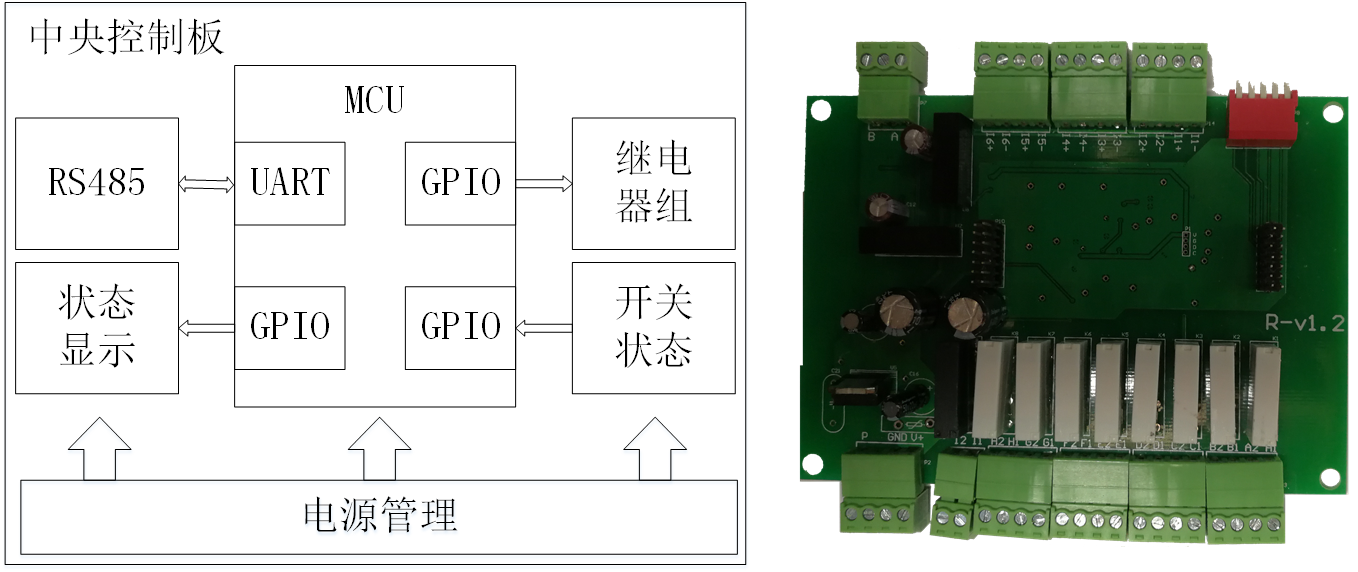
\includegraphics[width=0.8\textwidth]{09ControlBoard.png}
  			\bicaption[fig:ControlBoard]{中央控制板及其功能框图}{中央控制板及其功能框图}{Fig}{The photo and function diagram of the central control board}
		\end{figure}
	\subsection{图像采集模块}
图像采集部分采用HIKVISION CSC4S51WEFR网络摄像头,如\ref{fig:Camera}所示,接入图像采集网关可直接在局域网内对温室进行视频监控,如果温室现场网络条件良好,可接入云端服务生成m3u8视频流,提供在线视频观看,对于部分温室现场网络条件欠佳,本系统将通过定时采集现场静态图片的方式提供图像,同时接入云端图片存储服务,并返回对应URL。
	  	\begin{figure}[!htp]
  			\centering
 			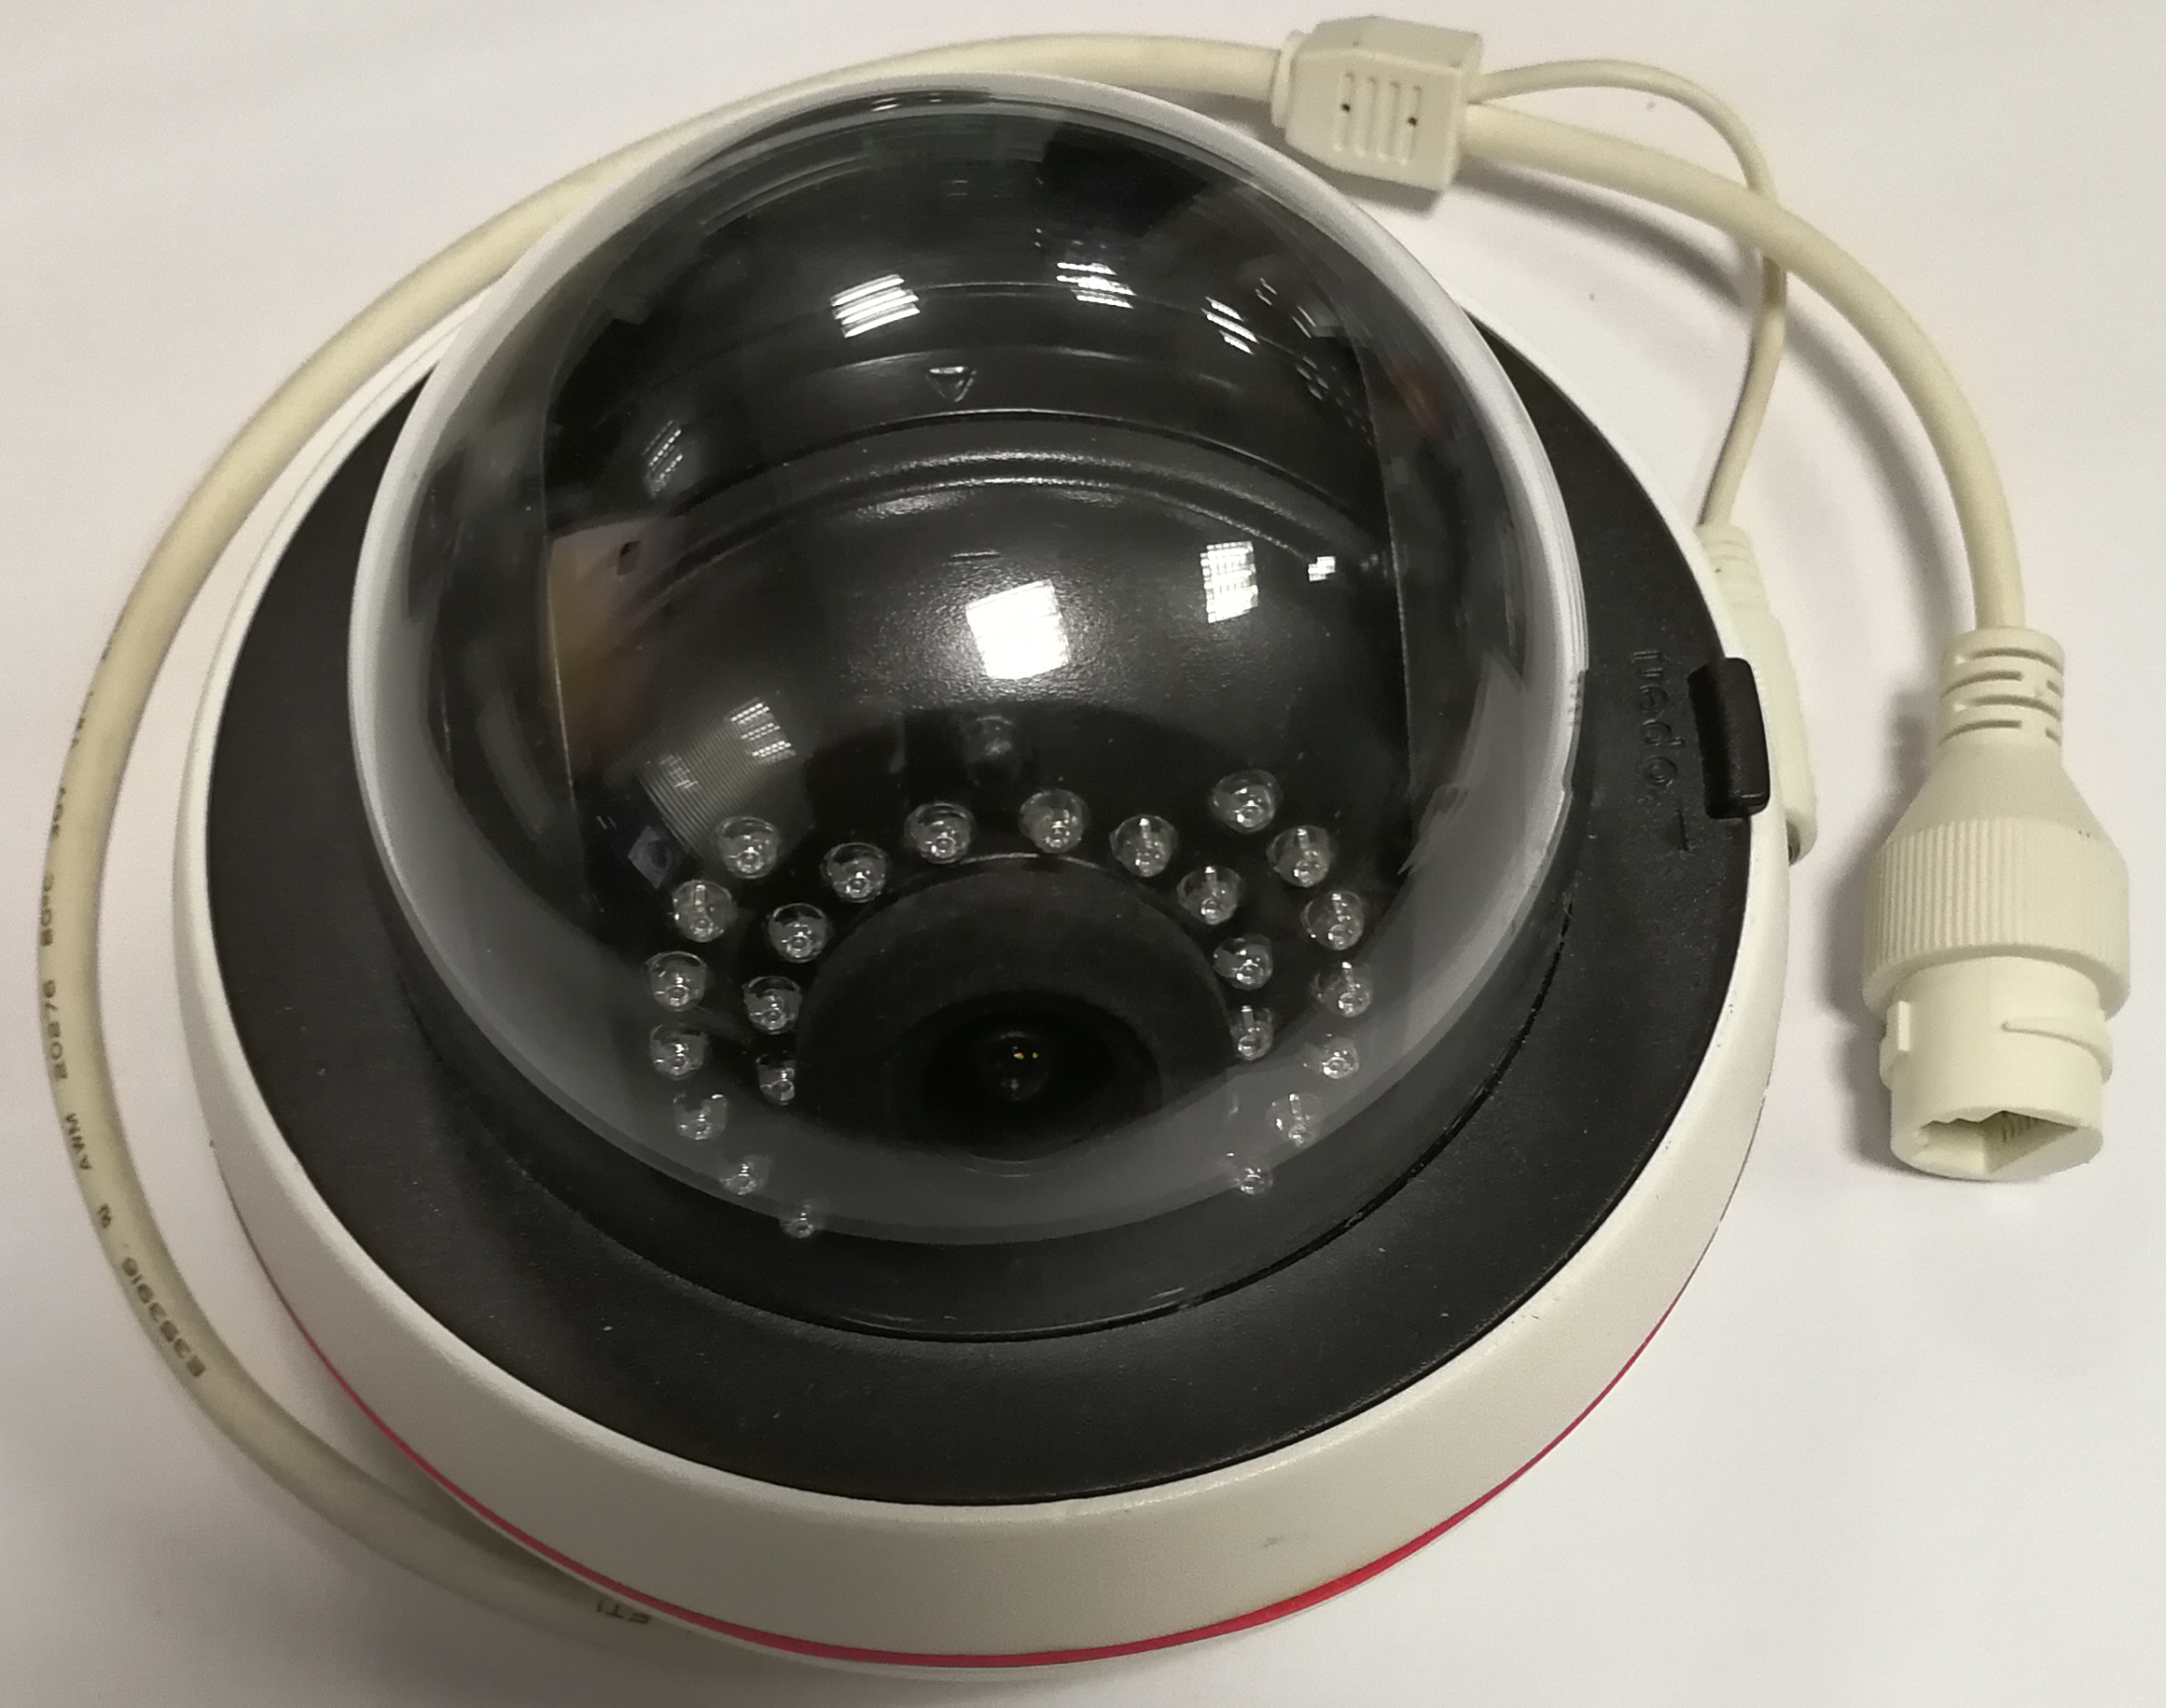
\includegraphics[width=0.8\textwidth]{10Camera.png}
  			\bicaption[fig:Camera]{HIKVISION CSC4S51WEFR网络摄像头}{HIKVISION CSC4S51WEFR网络摄像头}{Fig}{HIKVISION CSC4S51WEFR web camera}
		\end{figure}
\section{网络传输层设计与实现}
	\subsection{总体设计及技术简介}
	本文智能温室中的网络传输层通过数据传输与同步系统实现,该系统可实现控制指令和反馈信息的双向传输,以及传感器监测数据的上传与同步。其中监测数据的同步模块大部分部署在云端服务器,另一部分以及其余模块均部署运行在搭载Linux操作系统的基于ARM Cortex-A53的微型计算机上,该计算机具有64位4核CPU,主频为1.2 GHz,1 GB LPDDR2内存,最大支持64 GB内存卡,同时支持以太网连接和Wi-Fi连接,自带蓝牙4.1模块,4个USB接口,40个GPIO引脚,完全可满足现场计算服务的性能和通讯需求。
	
本系统内所有程序均采用Java语言编写,为进行串口通讯引入RXTX,使用Spring进行依赖注入管理和AOP编程,选择MyBatis作为数据持久化框架,数据库采用MySQL,未来将考虑使用更加轻量级、更加适用于嵌入式系统的SQLite代替MySQL作为现场数据存储数据库。

Java是一种功能强大且简单易用的面向对象编程语言,开源社区活跃,拥有众多优秀的开源框架和类库,可以快速便捷地开发各种跨平台的应用程序。RXTX是一个可开源Java串口库,具有良好的跨平台性,且向下兼容javax.comm串口库。Spring是一个轻量级的依赖注入管理和面向切面编程的容器框架,可以简化企业级Java应用的开发,极大地提高开发者的开发效率。MyBatis是一款开源的优秀持久层框架,使用简单的注解或配置,即可将通过接口将Java中的POJOs映射成数据库中的记录。MySQL是一款开源的非常轻量级的关系型数据库管理系统,功能强大,性能良好,且具有较小的体积,在世界范围内得到广泛的应用。

	\subsection{控制信息解析传输}
	系统中的控制指令和反馈信息的双向传输,通过控制信息解析传输程序实现,该程序部署在Tomcat容器中。
如\ref{fig:Control}所示,该程序的工作流程如下:
\begin{figure}[!htp]
    \centering
    \resizebox{6cm}{!}{\begin{tikzpicture}[node distance=2cm]
    \node (pic) [startstop] {开始};
    \node (bg) [io, below of=pic] {接收请求}; 
    \node (pair) [process, below of=bg] {匹配特征点对};
    \node (threshold) [decision, below of=pair, yshift=-0.5cm] {多于阈值};
    \node (clear) [decision, right of=threshold, xshift=3cm] {清晰?};
    \node (capture) [process, right of=pair, xshift=3cm, yshift=0.5cm] {重采};
    \node (matrix_p) [process, below of=threshold, yshift=-0.8cm] {透视变换矩阵};
    \node (matrix_a) [process, right of=matrix_p, xshift=3cm] {仿射变换矩阵};
    \node (reg) [process, below of=matrix_p] {图像修正};
    \node (return) [startstop, below of=reg] {配准结果};
     
    %连接具体形状
    \draw [arrow](pic) -- (bg);
    \draw [arrow](bg) -- (pair);
    \draw [arrow](pair) -- (threshold);

    \draw [arrow](threshold) -- node[anchor=south] {否} (clear);

    \draw [arrow](clear) -- node[anchor=west] {否} (capture);
    \draw [arrow](capture) |- (pic);
    \draw [arrow](clear) -- node[anchor=west] {是} (matrix_a);
    \draw [arrow](matrix_a) |- (reg);

    \draw [arrow](threshold) -- node[anchor=east] {是} (matrix_p);
    \draw [arrow](matrix_p) -- (reg);
    \draw [arrow](reg) -- (return);
\end{tikzpicture}
}
    \bicaption[fig:Control]{控制信息解析传输程序流程图}{控制信息解析传输程序流程图}{Fig}{Flow chart of control information transmission}
\end{figure}
程序向外暴露RESTful WebService接口,为了保证系统控制的安全性,避免恶意操作和非法操作等,系统会对所有请求的来源和合法性进行判断,所有接口仅向云端服务器开放,即如果该请求不是来自于指定的云端服务器,或者请求是非法的,均会被视为无效请求,将被立即拒绝并返回相应的错误信息。随后系统会对请求进行身份和权限鉴定,以避免误操作可能对温室设备带来的损坏,如果请求发起者没有相关操作的权限,请求将会被拒绝并返回相应的错误信息。随后系统根据不同的请求类型分别执行相应的动作,若操作成功则返回成功响应,否则返回响应的错误信息并向管理员发送告警通知。

	\subsection{数据采集上传}
	传感器网络的数据监测和同步上传,通过数据采集上传程序实现,程序的具体工作流程如下:
\begin{figure}[!htp]
    \subfigure[这是第一幅图]{
		\label{fig:Sampling:a} %% 第一幅图的标签
		\resizebox{6cm}{!}{\begin{tikzpicture}[node distance=2cm]
    \node (pic) [startstop] {开始};
    \node (bg) [io, below of=pic] {接收请求}; 
    \node (pair) [process, below of=bg] {匹配特征点对};
    \node (threshold) [decision, below of=pair, yshift=-0.5cm] {多于阈值};
    \node (clear) [decision, right of=threshold, xshift=3cm] {清晰?};
    \node (capture) [process, right of=pair, xshift=3cm, yshift=0.5cm] {重采};
    \node (matrix_p) [process, below of=threshold, yshift=-0.8cm] {透视变换矩阵};
    \node (matrix_a) [process, right of=matrix_p, xshift=3cm] {仿射变换矩阵};
    \node (reg) [process, below of=matrix_p] {图像修正};
    \node (return) [startstop, below of=reg] {配准结果};
     
    %连接具体形状
    \draw [arrow](pic) -- (bg);
    \draw [arrow](bg) -- (pair);
    \draw [arrow](pair) -- (threshold);

    \draw [arrow](threshold) -- node[anchor=south] {否} (clear);

    \draw [arrow](clear) -- node[anchor=west] {否} (capture);
    \draw [arrow](capture) |- (pic);
    \draw [arrow](clear) -- node[anchor=west] {是} (matrix_a);
    \draw [arrow](matrix_a) |- (reg);

    \draw [arrow](threshold) -- node[anchor=east] {是} (matrix_p);
    \draw [arrow](matrix_p) -- (reg);
    \draw [arrow](reg) -- (return);
\end{tikzpicture}
}
	}
    \subfigure[这是第一幅图]{
		\label{fig:Sampling:b} %% 第一幅图的标签
		\resizebox{6cm}{!}{\begin{tikzpicture}[node distance=2cm]
    \node (pic) [startstop] {开始};
    \node (bg) [io, below of=pic] {接收请求}; 
    \node (pair) [process, below of=bg] {匹配特征点对};
    \node (threshold) [decision, below of=pair, yshift=-0.5cm] {多于阈值};
    \node (clear) [decision, right of=threshold, xshift=3cm] {清晰?};
    \node (capture) [process, right of=pair, xshift=3cm, yshift=0.5cm] {重采};
    \node (matrix_p) [process, below of=threshold, yshift=-0.8cm] {透视变换矩阵};
    \node (matrix_a) [process, right of=matrix_p, xshift=3cm] {仿射变换矩阵};
    \node (reg) [process, below of=matrix_p] {图像修正};
    \node (return) [startstop, below of=reg] {配准结果};
     
    %连接具体形状
    \draw [arrow](pic) -- (bg);
    \draw [arrow](bg) -- (pair);
    \draw [arrow](pair) -- (threshold);

    \draw [arrow](threshold) -- node[anchor=south] {否} (clear);

    \draw [arrow](clear) -- node[anchor=west] {否} (capture);
    \draw [arrow](capture) |- (pic);
    \draw [arrow](clear) -- node[anchor=west] {是} (matrix_a);
    \draw [arrow](matrix_a) |- (reg);

    \draw [arrow](threshold) -- node[anchor=east] {是} (matrix_p);
    \draw [arrow](matrix_p) -- (reg);
    \draw [arrow](reg) -- (return);
\end{tikzpicture}
}
	}
    \bicaption[fig:Sampling]{数据采集上传程序流程图}{数据采集上传程序流程图}{Fig}{Flow chart of data sampling and uploading}
\end{figure}
首先程序将会去发现可用的串口设备,随后打开串口监听并保持,当监听到有效数据时将字节装入IO Buffer,如\ref{fig:Sampling:a}所示。

然后为了解决由于串口数据上传不完整而导致的数据包丢失问题,程序将同时启动如下四个线程,并采用生产者消费者的设计模式:
	\begin{enumerate}
		\item 串口读取线程。当串口IO Buffer中有缓存数据时,线程将从IO Buffer中读取字节流,并填入字节队列中,当IO Buffer无数据为空时,线程将阻塞等待。详细流程如\ref{fig:Sampling:b}所示。
		\item 数据打包线程。当字节队列中有数据时,线程从字节队列中读取字节并判断字节的类型:当读到包头字节即起始符时进入打包状态;当读到包尾字节即终止符时完成打包并对数据包进行校验,校验通过后装入数据包队列,否则丢弃并恢复普通状态;当读到其它字节时如果处于打包状态则将字节装入数据包,否则丢弃该字节。字节队列使用无限阻塞队列,意味着当字节队列为空时,线程继续从队列中获取对象将阻塞等待;如果队列中还存在未处理完成的字节时,读入的字节将添加在队列尾部。详细流程如\ref{fig:Sampling:b}所示。
		\item 数据包解析线程,当数据包队列中有数据包时,线程将从数据包队列中读取数据包并判断数据包的类型:当读到采集提示包时将向下层协调器发送数据采集指令;当读到数据包时则对数据包进行校验,校验通过后解析数据包并持久化到数据库,否则丢弃。数据包队列同样使用无限阻塞队列,数据包队列为空时,线程将阻塞等待。详细流程如\ref{fig:Sampling:b}所示。
		\item 采集指令发送线程,该线程会定时向室外气象站和太阳辐射强度传感器发送数据采集指令。
	\end{enumerate}
	
	\subsection{数据同步}
到目前为止所有的监测数据还都存储在温室群本地的现场微型计算机上,但是该现场微型计算机性能和存储空间有限,同时由于农业生产环境的限制,温室群所在地区网络环境一般较差,这给温室数据的远程获取带来了一定的阻碍,有可能会出现数据获取缓慢,甚至无法获取的情况,因此,本系统将所有监测数据同步到云端数据中心的数据库中,所有应用对于数据的获取将全部从云端数据库获取,这就解决了上述问题。
	  	\begin{figure}[!htp]
  			\centering
 			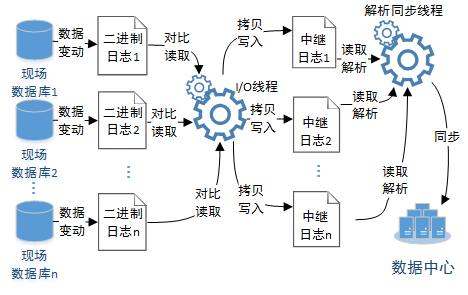
\includegraphics[width=0.8\textwidth]{11Sync.png}
  			\bicaption[fig:Sync]{数据同步过程}{数据同步过程}{Fig}{Process of the data synchronization}
		\end{figure}
监测数据的同步通过数据同步程序实现,如\ref{fig:Sync}所示,现场数据库在每个事务更新数据完成之前,会将这些事务串行地写入二进制日志中去,在事件日志写入完成之后将发出通知。随后云端同步程序将建立一个I/O线程对现场数据库的二进制日志文件进行订阅,当收到数据变动通知时将与现场数据库建立连接,随后将开始Binlog dump process从日志中读取相关事件,完成后将睡眠并等待通知,同时将事件写入中继日志,随后解析同步线程将提取中继日志中的事件进行解析并尝试向云端同步。

\section{应用及终端接入层设计与实现}
	本系统的数据中心和WEB服务器均部署和运行在云端服务器,具有高安全、高可用、灵活扩展、成本低等特点。
	\subsection{数据中心}
本系统的数据中心基于Hadoop构建,其中海量实时数据库使用HBase,数据仓库使用Hive,并使用MySQL作为近期历史数据的存储数据库。

Hadoop是一个分布式系统基础架构,可以对海量数据进行分布式的存储和处理,稳定可靠、易于扩展、性能突出、高度容错且成本低廉,是存储海量温室数据的较好的选择。HBase是一个面向列的NoSQL数据库,为了解决HDFS难以随机读写和缺乏实时性而出现。Hive是一个数据仓库工具,可以将SQL语句转换为MapReduce任务,极大程度地减少了开发人员的MapReduce jobs的编写工作。
	  	\begin{figure}[!htp]
  			\centering
 			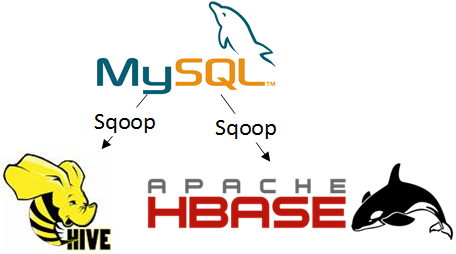
\includegraphics[width=0.8\textwidth]{12Data.png}
  			\bicaption[fig:Data]{ MySQL与Hive、HBase之间的迁移关系}{ MySQL与Hive、HBase之间的迁移关系}{Fig}{The relationship among MySQL and Hive/HBase}
		\end{figure}
数据中心通过MySQL接收下层系统同步上传的数据,以一个温室群布置30个终端节点和路由器节点,每10 min采集一组数据为例,仅传感监测数据每天可产生2.2×104条记录,每年可产生 8×106条记录,室外气象参数监测每天也将产生大量的数据,同时温室控制每天还将产生大量控制日志记录,这样一个温室群每年将产生数千万条数据,多个温室群每年将产生数亿条数据,这会严重影响MySQL工作效率,虽然进行分库分表操作可一定程度上缓解这种问题,但是将增加数据库复杂度,而且考虑到在实际生产中,经常访问的均为近期的监测数据,大量历史数据仅需用于后期的查询、导出和分析。因此,本系统定期地将把MySQL中历史数据通过Sqoop工具迁移至HBase和Hive中保存,迁移关系如\ref{fig:Data}所示,MySQL数据库中仅保存温室近期数据。HBase和Hive中的历史数据将用于后期数据分析和控制策略的机器学习。
 
	\subsection{WEB服务器}
温室环境监测数据采集完成并同步到云端的数据中心,系统还需要向外界提供相关的服务,包括提供温室环境远程监测查看、温室环境远程控制、温室现场视频或图像查看等服务,因此需要WEB服务器及其相关服务端程序。

本系统选用商用云服务器作为WEB服务器,可提供7×24小时不间断服务保证,简单高效,处理能力和存储空间可弹性伸缩,免除了机房维护的问题,降低了运维成本。服务器上运行64位CentOS 6.5操作系统,CentOS是当今最流行的服务端Linux发行版之一,由Red Hat Enterprise Linux依照开放源代码规定公布出的源代码编译而成,具有高度的稳定性和可靠性、良好的性能,因此非常合适作为服务端操作系统。
	  	\begin{figure}[!htp]
  			\centering
 			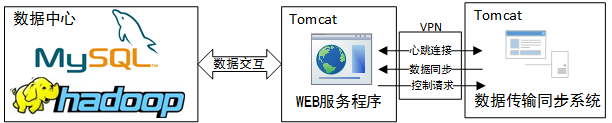
\includegraphics[width=0.8\textwidth]{13Web.png}
  			\bicaption[fig:Web]{WEB服务程序工作流程}{WEB服务程序工作流程}{Fig}{Workflow of the webservice}
		\end{figure}
WEB服务端程序均部署在Tomcat容器中,全部使用Java语言编写,基于典型SSM框架开发,即Spring + Spring MVC + MyBatis框架,采用MVC(Model View Controller)分层设计模型,其中Spring为程序提供必要的依赖注入和AOP框架,Spring MVC作为程序的轻量级请求驱动的WEB应用框架,可以方便地实现MVC模型,MyBatis则为程序提供了数据持久层框架。
 
WEB服务程序工作流程如\ref{fig:Web}所示。所有数据均与数据中心进行交互。考虑到安全因素,保证系统的安全性,服务器向下通过VPN(Virtual Private Network)连接数据传输与同步系统,可调用控制接口对温室设备进行控制,接收数据同步请求进行数据同步,同时建立心跳连接以确定与下层系统的网络连通状态,以便于及时通知系统管理人员当前系统的状态。同时向外暴露RESTful WebService接口,供终端程序调用并返回JSON格式数据,实现前后端分离设计,也可为其它接入的系统提供相关服务。

	\subsection{智能策略学习控制子系统}
智能温室监测与控制不仅要解决温室内环境远程监测与远程控制的问题,更进一步是要解决温室的智能控制,即温室在不需要人工参与的情况下可以实现自主根据当前的温室环境参数,控制温室各种可用作动器的单独动作或组合动作,完成温室环境的控制调节。

温室是一个流场、温度场、浓度场等多物理场耦合在一起的多输入多输出的大时延系统,对温室任何目标的控制,都会影响到其它状态的变化,且对于外界所施加的作用,温室都会经过一段延时后才会有所响应。这些因素都导致温室环境控制是一个极其复杂和困难的问题。为了解决温室控制的问题,本系统采用专家经验提供初始策略,CFD仿真模拟提供优化分析建议,机器学习模型持续训练迭代的方式。

传统的温室环境控制多依靠农业生产人员以及专家的经验来进行,但是中国幅员辽阔,地区差异极大,每个温室又各不相同,经验往往是有针对性的,难以适应不同温室的控制需求。针对以上这些问题,本系统设计了智能策略学习控制子系统,该子系统根据专家经验制定初始的控制策略,通过CFD仿真技术和机器学习技术,实现温室环境控制策略的优化,以及控制策略后期的自主学习,不断完善控制策略,改善控制效果。

借助CFD仿真技术可以更加清晰、定量化地了解温室的结构参数、作动器的不同动作组合、温室内外的环境参数对于温室环境参数变化和分布的影响。根据经过验证的温室CFD模型,系统可以得到任意环境条件下,任意温室内的任意作动器动作引起的温室环境的变化和分布,通过稳态和瞬态的分析,不仅可以了解控制效果,还可以了解其变化过程,这些都可以帮助更好地优化控制策略,改善控制效果,同时减少能源消耗。

机器学习技术可以让系统控制策略根据温室环境的历史数据、温室控制日志的历史数据和温室作动器的不同控制组合不断更新迭代已有的控制策略,实现温室控制策略的自主学习和自适应学习。系统可采用K-means算法对温室环境的历史数据进行聚类并按照规则打分,然后利用改进的Apriori聚类分析算法对控制日志历史数据、控制组合和已分类的温室环境历史数据进行聚类找出其中最有的组合并根据结果决定是否更新当前控制策略。

	\subsection{终端程序}
终端程序分为WEB页面程序和移动终端程序,均可接入智能温室系统的应用层,实现温室远程监测和控制,以及温室现场的图像与视频监控。

所有前端程序均部署在云端Nginx服务器,该服务器资源消耗小,并发能力强,稳定性高,有丰富的功能集,且高度可配置。

WEB页面使用HTML5 + CSS3 + JavaScript开发,使用Node.js作为JavaScript开发运行环境,主要使用的技术栈有React、Redux、Webpack和Sass,使用React Router作为前端路由器库,通过AJAX技术调用应用层所提供的接口,得到JSON数据,并将数据按照自定格式解析后展示到页面。

其中Node.js是一个基于Chrome V8 引擎的轻量高效的JavaScript 运行环境。React是Facebook开源的一款前端JavaScript MVC框架,主要解决View层的开发,官方给它的定义是一套用来生成用户界面的JavaScript库,为了配合React开发,前端选用React Router作为路由库,用以管理资源路径,实现组件的切换和状态的变化。为了确保前端页面状态的可预测性,使用Redux作为前端页面容器。Webpack 是目前非常流行的开发便捷、扩展性强的前端资源模块加载器和打包工具,利用Webpack可以按照依赖关系和相关规则将松散的模块打包成符合生产环境部署的前端资源,还可以将按需加载的模块进行代码分隔,等到实际需要的时候再异步加载,通过加载器的转换,不仅仅是JS,任何形式的前端资源都可以视作模块,比如ES6模块、CSS、图片、JSON等。Sass是一种成熟、稳定而且非常强大的专业级CSS扩展语言,完全兼容CSS语法,同时提供了许多便利的写法,大大节省了设计者的时间,使得CSS的开发,变得简单和易维护。AJAX即“Asynchronous JavaScript And XML(异步JavaScript和XML)”,是指一种用来创建交互式网页应用的网页开发技术,它使得页面可以异步更新,即只对其中的局部进行刷新而无需全部重新刷新。JSON(JavaScript Object Notation) 是一种数据交换格式,在让人可以非常容易读写的同时还非常便于机器的解析生成。

移动客户端使用React Native开发,React Native同样是Facebook开源的一套前端应用技术框架,开发者通过React Native可利用JS和React创建原生移动应用,并且可复用大部分代码同时生成Android平台和IOS平台应用。移动应用同样调用应用层提供的接口获得返回数据,然后经过解析展示到界面。
	  	\begin{figure}[!htp]
  			\centering
 			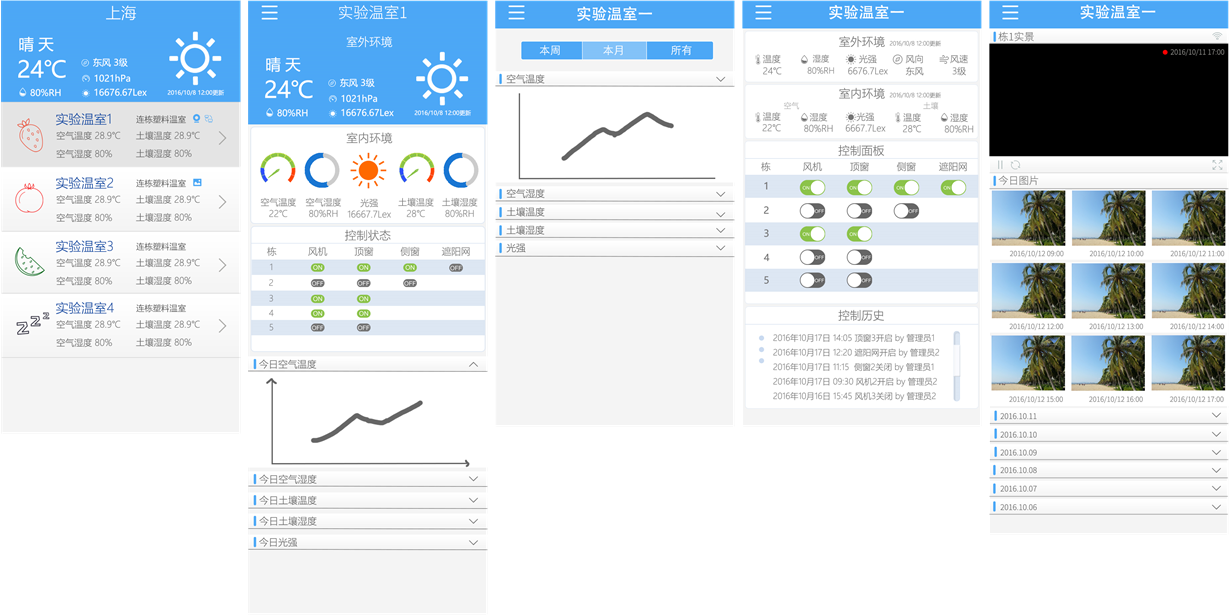
\includegraphics[width=0.8\textwidth]{14Design.png}
  			\bicaption[fig:Design]{终端程序界面设计}{终端程序界面设计}{Fig}{UI design of the terminal program}
		\end{figure}
本次系统所有终端程序,包括WEB页面和移动客户端应用,均使用相同的UI和功能设计,设计图如\ref{fig:Design}所示,主要分为温室选择页、温室详情页、历史曲线页、温室控制页、温室实景页等页面。

温室选择页,如\ref{fig:Design}所示,用以显示所有的温室,并可选择任意温室进入。该页面上部可以查看当前温室地区的天气情况,下部列出所有的温室,并显示温室当前种植的作物图标、温室名称、温室类型、是否可以远程控制、是否有视频服务、是否有图像服务,以及温室当前的室内环境概况。

温室详情页,如\ref{fig:Design}所示,用以显示所查看温室内的详细情况。该页面上部可查看当前温室室外环境参数,然后是温室室内的环境参数,若温室可控制则会显示温室作动器的控制状态,最下部显示温室当天的室内环境参数曲线。

历史曲线页,如\ref{fig:Design}所示,该页显示温室一周内、一月内和所有近期的室内参数历史数据曲线,目前仅可查询一年内的数据曲线。

温室控制页,如\ref{fig:Design}所示,如果温室可远程控制,则温室控制页可用,否则该页不可进入,用于远程控制温室内的作动器。该页面上部分别显示温室外和温室内的环境参数,中间为用于远程控制的按钮,下部为当前温室的控制历史日志。

温室实景页,如\ref{fig:Design}所示,用于查看温室的当前视频和图像。如果温室视频服务可用的话则上部显示视频播放窗口,否则不显示;如果温室图像服务可用的话则显示近七天的图片,否则不显示,该部分图片既可以是温室摄像头自动捕获,也可以是人工上传;如果温室视频服务和图像服务都不可用则该页面不可进入。
	\subsection{本章小结}
本章按照系统架构设计的层次划分,以及各层次的概要设计,对每个层次进行了详细的设计,并基本实现完成。

感知控制层设计实现了传感器网络,包括硬件的设计和选型、传感器的选型、无线传感器网络的自定义协议及流程,同时对无线传感器网络节点进行了低功耗优化,使其能够满足农业生产环境恶劣、不易值守的特殊需求。另外完成了控制模块的硬件设计和选型,以及视频图像采集模块的设计和选型。

网络传输层主要实现了控制信息解析传输程序、数据采集上传程序和数据同步程序,搭建了感知控制层和上层系统之间的桥梁,使得温室环境监测数据能够稳定高效地采集并同步上传,控制指令能够稳定及时地下发。

应用层和终端接入层在商用云端服务器上搭建并配置了所需要的服务器端运行环境;基于Hadoop和MySQL搭建了农业物联网数据中心,解决了海量农业数据的存储和数据访问问题;使用Linux + Tomcat + Java的运行环境,基于Spring + Spring MVC + MyBatis的J2EE框架,构建了完整的服务器端程序;综合运用CFD仿真技术和机器学习技术设计了智能控制策略学习控制子系统,优化温室环境控制策略,以实现智能温室系统对温室环境的智能控制;使用Linux + Nginx的运行环境,基于HTML5 + CSS3 + JavaScript + AJAX技术构成,综合运用React、Redux、Webpack和Sass等技术,实现终端程序中WEB页面的开发,同时使用React Native实现移动端应用的开发,包括Android端和IOS端应用。
